\documentclass[tikz,border=10pt]{standalone}
\usepackage{tikz}
\usetikzlibrary{shapes,arrows,positioning,decorations.pathreplacing,backgrounds,fit,shadows,calc}

% Define colors
\definecolor{inputblue}{RGB}{66,133,244}
\definecolor{processgreen}{RGB}{52,168,83}
\definecolor{llmorange}{RGB}{255,152,0}
\definecolor{outputpurple}{RGB}{156,39,176}
\definecolor{stream1color}{RGB}{30,136,229}
\definecolor{stream2color}{RGB}{0,150,136}
\definecolor{stream3color}{RGB}{121,85,72}

% Define styles
\tikzstyle{inputbox} = [rectangle, rounded corners=5pt, minimum width=3.2cm, minimum height=1.2cm, text centered, draw=inputblue!80, fill=inputblue!20, text width=2.8cm, font=\small\bfseries, drop shadow]
\tikzstyle{processbox} = [rectangle, rounded corners=5pt, minimum width=2.8cm, minimum height=1cm, text centered, draw=processgreen!80, fill=processgreen!20, text width=2.5cm, font=\small]
\tikzstyle{llmbox} = [ellipse, minimum width=2.8cm, minimum height=0.7cm, text centered, draw=llmorange!90, fill=llmorange!30, font=\tiny\bfseries, drop shadow]
\tikzstyle{outputbox} = [rectangle, rounded corners=5pt, minimum width=3.2cm, minimum height=1.2cm, text centered, draw=outputpurple!80, fill=outputpurple!20, text width=2.8cm, font=\small\bfseries, drop shadow]
\tikzstyle{arrow} = [thick,->,>=stealth, color=black!70]
\tikzstyle{arrowdashed} = [thick,->,>=stealth,dashed, color=llmorange!80]

\begin{document}
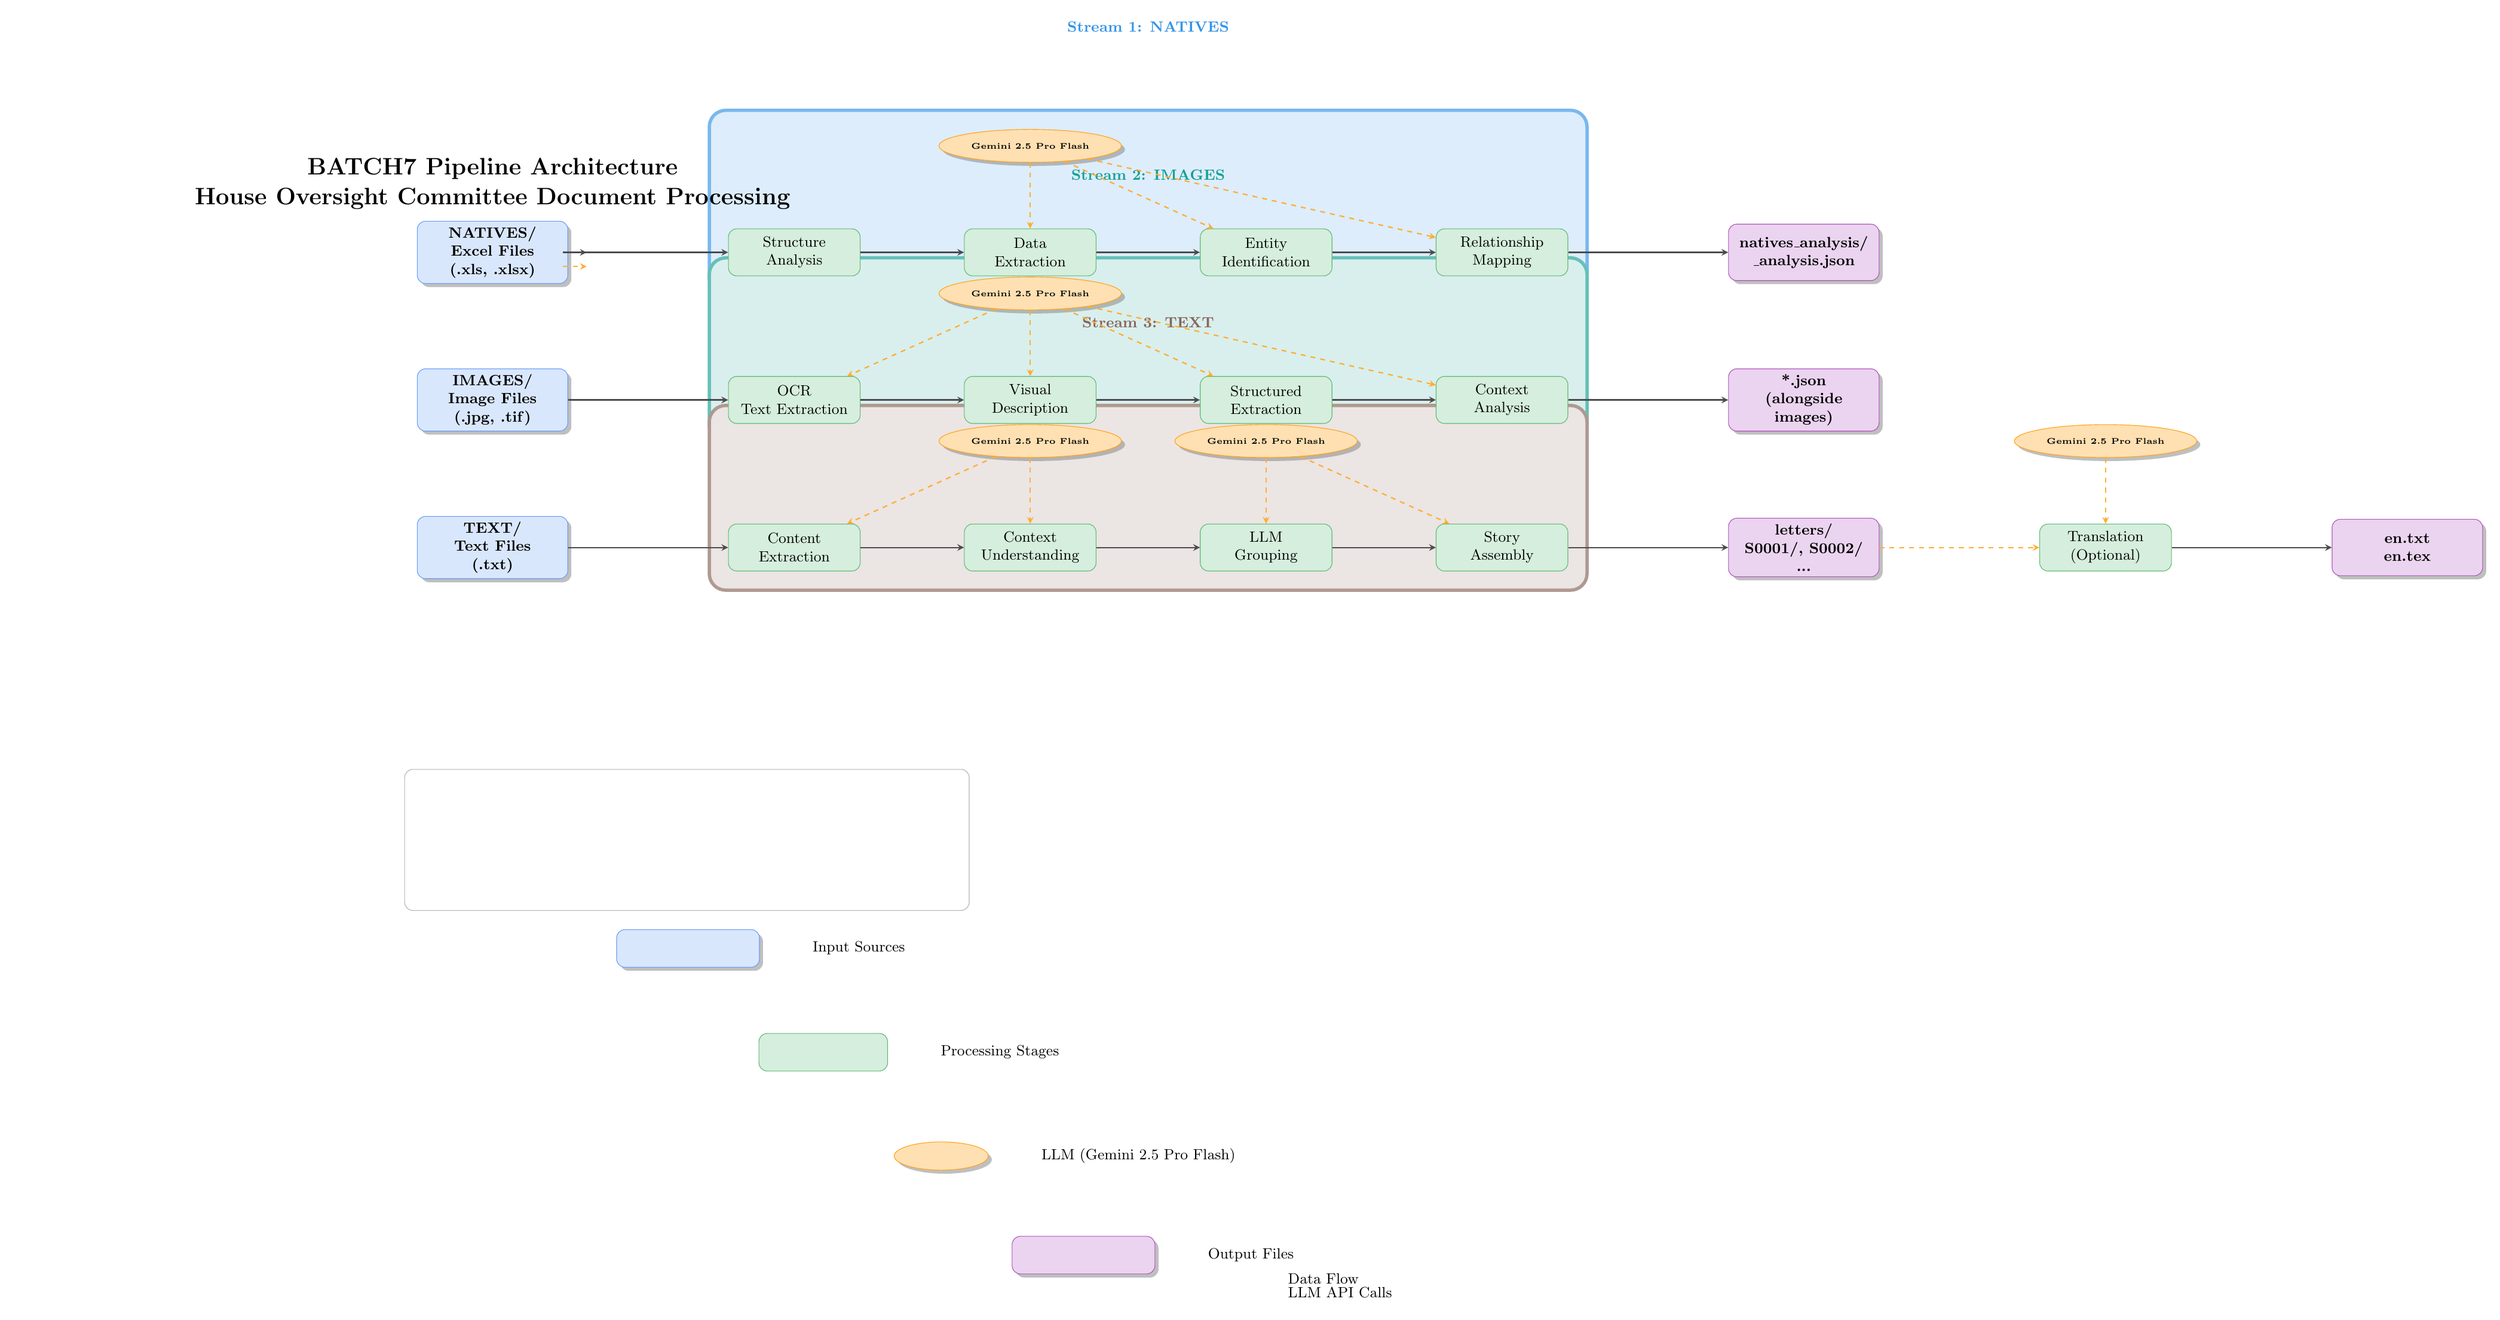
\begin{tikzpicture}[node distance=1.8cm and 2.2cm]

% Title
\node[above, font=\Large\bfseries, yshift=0.8cm, text width=20cm, align=center] (title) {BATCH7 Pipeline Architecture\\House Oversight Committee Document Processing};

% Input layer
\node[inputbox] (natives) {NATIVES/\\Excel Files\\(.xls, .xlsx)};
\node[inputbox, below=of natives] (images) {IMAGES/\\Image Files\\(.jpg, .tif)};
\node[inputbox, below=of images] (text) {TEXT/\\Text Files\\(.txt)};

% Stream 1: NATIVES Processing
\node[processbox, right=of natives, xshift=1.2cm] (n1) {Structure\\Analysis};
\node[processbox, right=of n1] (n2) {Data\\Extraction};
\node[processbox, right=of n2] (n3) {Entity\\Identification};
\node[processbox, right=of n3] (n4) {Relationship\\Mapping};
\node[llmbox, above=of n2, yshift=-0.4cm] (llm1) {Gemini 2.5 Pro Flash};

% Stream 2: IMAGES Processing
\node[processbox, right=of images, xshift=1.2cm] (i1) {OCR\\Text Extraction};
\node[processbox, right=of i1] (i2) {Visual\\Description};
\node[processbox, right=of i2] (i3) {Structured\\Extraction};
\node[processbox, right=of i3] (i4) {Context\\Analysis};
\node[llmbox, above=of i2, yshift=-0.4cm] (llm2) {Gemini 2.5 Pro Flash};

% Stream 3: TEXT Processing
\node[processbox, right=of text, xshift=1.2cm] (t1) {Content\\Extraction};
\node[processbox, right=of t1] (t2) {Context\\Understanding};
\node[processbox, right=of t2] (t3) {LLM\\Grouping};
\node[processbox, right=of t3] (t4) {Story\\Assembly};
\node[llmbox, above=of t2, yshift=-0.4cm] (llm3) {Gemini 2.5 Pro Flash};
\node[llmbox, above=of t3, yshift=-0.4cm] (llm4) {Gemini 2.5 Pro Flash};

% Output layer
\node[outputbox, right=of n4, xshift=1.2cm] (o1) {natives\_analysis/\\*\_analysis.json};
\node[outputbox, right=of i4, xshift=1.2cm] (o2) {*.json\\(alongside images)};
\node[outputbox, right=of t4, xshift=1.2cm] (o3) {letters/\\S0001/, S0002/\\...};

% Optional translation
\node[processbox, right=of o3, xshift=1.2cm] (trans) {Translation\\(Optional)};
\node[llmbox, above=of trans, yshift=-0.4cm] (llm5) {Gemini 2.5 Pro Flash};
\node[outputbox, right=of trans, xshift=1.2cm] (o4) {en.txt\\en.tex};

% Arrows - Stream 1 (NATIVES)
\draw[arrow] (natives) -- (n1);
\draw[arrow] (n1) -- (n2);
\draw[arrow] (n2) -- (n3);
\draw[arrow] (n3) -- (n4);
\draw[arrow] (n4) -- (o1);
\draw[arrowdashed] (llm1) -- (n2);
\draw[arrowdashed] (llm1) -- (n3);
\draw[arrowdashed] (llm1) -- (n4);

% Arrows - Stream 2 (IMAGES)
\draw[arrow] (images) -- (i1);
\draw[arrow] (i1) -- (i2);
\draw[arrow] (i2) -- (i3);
\draw[arrow] (i3) -- (i4);
\draw[arrow] (i4) -- (o2);
\draw[arrowdashed] (llm2) -- (i1);
\draw[arrowdashed] (llm2) -- (i2);
\draw[arrowdashed] (llm2) -- (i3);
\draw[arrowdashed] (llm2) -- (i4);

% Arrows - Stream 3 (TEXT)
\draw[arrow] (text) -- (t1);
\draw[arrow] (t1) -- (t2);
\draw[arrow] (t2) -- (t3);
\draw[arrow] (t3) -- (t4);
\draw[arrow] (t4) -- (o3);
\draw[arrowdashed] (llm3) -- (t1);
\draw[arrowdashed] (llm3) -- (t2);
\draw[arrowdashed] (llm4) -- (t3);
\draw[arrowdashed] (llm4) -- (t4);

% Translation arrows
\draw[arrowdashed] (o3) -- (trans);
\draw[arrow] (trans) -- (o4);
\draw[arrowdashed] (llm5) -- (trans);

% Background boxes for streams with different colors
\begin{scope}[on background layer]
    \node[fill=stream1color!15, rounded corners=10pt, fit=(n1)(n4)(llm1), inner sep=0.4cm, draw=stream1color!60, line width=2pt] (stream1) {};
    \node[fill=stream2color!15, rounded corners=10pt, fit=(i1)(i4)(llm2), inner sep=0.4cm, draw=stream2color!60, line width=2pt] (stream2) {};
    \node[fill=stream3color!15, rounded corners=10pt, fit=(t1)(t4)(llm3)(llm4), inner sep=0.4cm, draw=stream3color!60, line width=2pt] (stream3) {};
    
    % Labels for streams
    \node[font=\small\bfseries, text=stream1color!90, above=of stream1, yshift=-0.3cm] {Stream 1: NATIVES};
    \node[font=\small\bfseries, text=stream2color!90, above=of stream2, yshift=-0.3cm] {Stream 2: IMAGES};
    \node[font=\small\bfseries, text=stream3color!90, above=of stream3, yshift=-0.3cm] {Stream 3: TEXT};
\end{scope}

% Legend box
\node[below=of text, yshift=-2cm, anchor=north west, font=\small] (legend) {};
\node[rectangle, rounded corners=5pt, fill=white!90, draw=black!30, below=of legend, yshift=0.3cm, anchor=west, xshift=-2cm, minimum width=12cm, minimum height=3cm] (legendbox) {};

% Legend items
\node[inputbox, below=of legendbox, yshift=1cm, anchor=west, xshift=-1.5cm, minimum width=2cm, minimum height=0.8cm] (leg1) {};
\node[right=of leg1, xshift=-1.2cm, font=\small] {Input Sources};

\node[processbox, below=of leg1, anchor=west, xshift=1.5cm, minimum width=2cm, minimum height=0.8cm] (leg2) {};
\node[right=of leg2, xshift=-1.2cm, font=\small] {Processing Stages};

\node[llmbox, below=of leg2, anchor=west, xshift=1.5cm, minimum width=2cm, minimum height=0.6cm] (leg3) {};
\node[right=of leg3, xshift=-1.2cm, font=\small] {LLM (Gemini 2.5 Pro Flash)};

\node[outputbox, below=of leg3, anchor=west, xshift=1.5cm, minimum width=2cm, minimum height=0.8cm] (leg4) {};
\node[right=of leg4, xshift=-1.2cm, font=\small] {Output Files};

% Legend arrows
\draw[arrow, below=of leg4, anchor=west, xshift=1.5cm] (0,0) -- (0.5,0);
\node[right=of leg4, xshift=0.5cm, yshift=-0.5cm, font=\small] {Data Flow};

\draw[arrowdashed, below=of leg4, anchor=west, xshift=1.5cm, yshift=-0.3cm] (0,0) -- (0.5,0);
\node[right=of leg4, xshift=0.5cm, yshift=-0.8cm, font=\small] {LLM API Calls};

\end{tikzpicture}
\end{document}

